\documentclass{article}
\usepackage{v-problem}
\vgeometry[5][5]

\begin{document}
\vtitle[RAY-OPTICS]

\def\pn{01}
\def\exam{IIT-JEE}
\def\year{2022}
\def\gdrive{https://drive.google.com/drive/folders/1fbX85gQQ_sRVL4y8QF0D0ZvCSbL-BOiu?usp=share_link}

\def\question{
A rod of length $2\cm$ makes an angle $\dfrac{2\pi}{3}$ with the principal axis of a thin convex lens. The lens has a focal length of $10\cm$ and is placed at a distance of $\dfrac{40}{3}\cm$ from the object as shown in the figure. The height of the image is $\dfrac{30\sqrt{3}}{13}\cm$ and the angle made by it with respect to the principal axis is $\alpha$. The value of $\alpha$ is $\dfrac{\pi}{n}$, where $n$ is 
}

\def\option{
\begin{tasks}(2)
\task $\dfrac{b^2\tau}{4}$
\task $\dfrac{b^2\tau}{2}$
\task $b^2\tau$
\task $\dfrac{b^2\tau}{\sqrt{2}}$
\end{tasks}
}

\vspace*{\fill}
\begin{tikzpicture}
	\node[qnumber] (n) at (0, 0)[scale=2] {$\pn.$};
	\node[question] (q) [right=2mm of n.east] {\question};
	\tzline[divider]<-0.125, 0> (q.north west)(q.south west);
	\node[format] (f) at  (q.south east){[\exam \quad \year]};
\end{tikzpicture}	
\vspace*{\fill}

\begin{center}
\begin{tikzpicture}
[thick, scale=0.7, cap=round]
	\tzline(-7, 0)(7, 0)
	\tzellipse(0, 0)(0.4cm and 3cm)
	\tzline+[ultra thick] (-5, 0)(120:1)
	\tzanglemark(0, 0)(-5, 0)($(-5, 0)+(120:1)$){$\dfrac{2\pi}{3}$}[r]
	\tzline+[ultra thick] (6, 0)(-120:2)
	\tzanglemark(0, 0)(6, 0)($(6, 0)+(-120:2)$){$\alpha$}
	\tzline[|<->|]<0, -0.5>(-5, 0)(0, 0){$\dfrac{40}{3}$}[mb]
	\tzline+[|<->|]<-0.5, 0>($(6, 0)+(-120:2)$)(0, 2*sin{60}){$\dfrac{30\sqrt{3}}{13}$}[ml]
\end{tikzpicture}
\end{center}
\pagebreak

\vspace*{\fill}
\begin{center}
	\fbox{\qrcode[height=2cm]{\gdrive}}
\end{center}
\vspace*{\fill}

\end{document}
